\chapter{Problem Analysis And Solution}

In this chapter, we will discuss the decisions we made during application design and reasons behind every choice. We will define what influenced the chosen application structure. Finally, we will explain the purpose of each part of the application.

%%-----------------------------------------------------------------------------------------
%% SECTION
%%-----------------------------------------------------------------------------------------
\section{Main Features}
At the beginning of the design we decided to establish three main features that would help us create a successful application. Each of them should give us an advantage over current or future competition as well as reduce the amount of work needed compared to establishing them in the later parts of design and development.

%%-----------------------------------------------------------------------------------------
\subsection{Multi-platform Application}

First step on the way to create any piece of software is to select target platform. There are three main platforms, Microsoft's Windows leading the market share with a big margin to Apple's OS X then followed by Linux (see Fig. \ref{fig01:osMarketShareChart}).

\begin{figure}[h]\centering
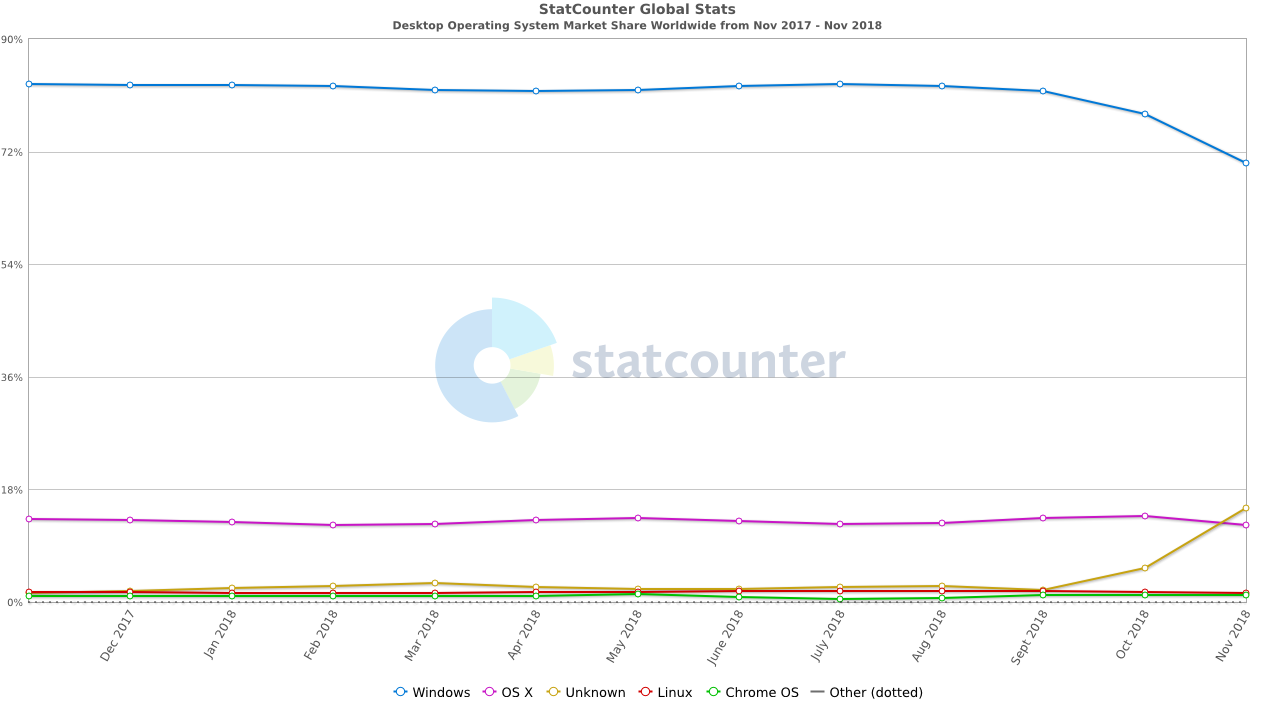
\includegraphics[width=1.0\textwidth]{img/StatCounter-os_combined-ww-monthly-201711-201811}
\caption{Desktop Operating System Market Share Worldwide from Nov 2017 - Nov 2018~\citep{osMarketShare}}
\label{fig01:osMarketShareChart}
\end{figure}

For simplicity we could assume that vast majority of users use Windows and we could target this single platform without losing many potential users. But we don't know the exact market share in our target group and focusing on single platform may be a big mistake.
\par
Another reason to support multiple platforms is the recent progress of miniature PCs. The most important task of our application is to play music and these computers have enough computing power to do that and require just a small initial investment into hardware that would do so. These PCs usually run or at least support modified versions of Linux, which has the smallest market share among major operating systems.
\par
The downside to this is the obvious extra amount of work that needs to be done both during analysis and subsequent implementation. However, we consider the benefits of adopting this feature early to be significant enough compared to the risk of having to support additional platform after the implementation is finished.
%%-----------------------------------------------------------------------------------------
\subsection{Modular Design}

If we could divide our application into reasonable amount of modules and define exact interface and relationship among them, the resulting design would have a lot of flexibility both from user's and developer's point of view.
\par
As developers, we would be able to make best decisions regarding each module without having to worry about other modules as long as we keep the predefined interface. We can create specialized versions of one module without having to modify any other. Furthermore, no two modules have to run on the same machine, in the same building or even the same country.
\par
Instead of having one monolithic application, our users may select suitable modules for their needs and customize it to their needs. Every use case has its specifics and adopting this feature allows us to offer each user a suitable solution.
\par
Being bound by predefined interfaces is a drawback that we must face, so they must be designed with extra care and robustness in order to be beneficial.
%%-----------------------------------------------------------------------------------------
\subsection{Scalability}

The last fundamental feature is scalability. We have set a goal to attract a wide range of users, so our application must be able to function properly with any size of music library and any number of regular users wanting to listen to their favourite song. Having adopted modular design earlier, we can achieve scalability also by offering a more capable module as a replacement for one that has reached its maximum potential. Nevertheless, all modules should only be limited by computing power provided by the user.

%%-----------------------------------------------------------------------------------------
%% SECTION
%%-----------------------------------------------------------------------------------------
\section{Programming Language}

Next decision we had to take was to select a suitable programming language. We had to satisfy the main features and their demands that we have set earlier. That is, we had to find a way to support multiple platforms, while in the same time we needed flexible enough language to handle our modular design and fast enough to help us with scalability.
\par
One solution would be to create an implementation for every platform in a language that is native for them. That would probably result in use of C++ and a Linux-friendly UI framework on Linux, Objective-C on macOS and C\# on Windows. While this would allow us to create suitable application for each platform and to use platform-specific frameworks and libraries, it would be highly labour-intensive as it would require every piece of code to be written three times. Furthermore, it would require knowledge of all three programming languages. Therefore we declined this solution because it offered too little benefits at too high price.
\par
Another way would be to use a language that was designed to be multi-platform like Java. We would only need to write code once and then run it on all three platforms. We had to reject this solution for two reasons. First is the core problem of Java - it requires a Java Virtual Machine to run any Java code, which might be a big penalty in our goal to make our application available on miniature PCs. Second reason is the struggle with UI frameworks that Java offers. While they might have improved over the past few years and might be suitable for business applications, we want to create an application with attractive and modern UI and we do not think Java can offer this. Another language with such capabilities would be C++, but we have to reject it for the same UI framework issues.  
\par
We could try to improve the above solutions. What we needed to realize is that the major problem on each platform was the user interface. That is the major thing that disallows us to use one language across all platforms. With that in mind we can create a solution where the backend - the logic of the application and IO management - would be written in C++ and we would use bindings that Objective-C and C\# offer to call code written in C++. Then we would only need to implement the UI for each platform. This way the amount of code, that would need to be written multiple times, would be significantly reduced. However, we would still need to know all three languages in order to do so.
\par
What we wanted to achieve is to write every piece of code just once. Here we applied my knowledge gained while working on my semestral project. There the whole UI was written in HTML5 and JavaScript. These two technologies are used all around the Internet and web apps have seen a great rise in popularity. It benefits us because it means that there are numerous good frameworks available and users would be used to an application designed in a similar manner. Then we would need to write the UI just once and it would look the same across all platforms.
\par
It turns out that the above-mentioned ideas are now feasible. There is an open-source project written in C++ called Chromium Embedded Framework~(CEF). CEF focuses on facilitating embedded browser use cases in third-party applications~\citep{cef}. That means that we can embed a web browser in our application where we run the UI and the rest of the backend will run alongside that. CEF offers a way to call C++ code from JavaScript so we do not need to worry about communication between these two languages.
%\todo{write a paragraph about previous project on electron and that we found CEF and that identical UI benefits us}

%%-----------------------------------------------------------------------------------------
%% SECTION
%%-----------------------------------------------------------------------------------------
\section{Modules}

In this section we will talk about all the modules that we decided to divide our application into. We will explain why we need each module, what is their role and purpose and how they communicate between each other.
\par
First, we need to understand what functionality our application requires. Then we can group similar functionality together and wrap it up in modules. Each module should be able to perform its task without the help of another and offer certain services to other modules or be able to consume other module's services if needed. These services will then be predefined by a certain interface so we gain an ability to work with different implementations of on module without the need to modify other modules.
\par
We need to have access to a collection of music files, keep information about their location, store their metadata like title, artist, album for easier browsing and allow to group them into playlists. Usually, this is called music library.
\par
Then we need to be able to play these music files. In order to do that, first we need to access them. Most music files are encoded to use less storage space, so we need to decode them. Only then we can send the data to sound card to finally play some music.
\par
We will also need to allow our users to browse the music library. Let them order the songs and create their playlists. Give them control over music playback. Allow them to customize the application and set the settings they need. Show them what regular users ordered to be played. We require our UI to support all of this.
\par
Lastly, we need a tool for synchronization between our application and the regular users. They want to see what songs we offer in our playlist and we want to know their orders so we can play what they desire.
\par
Above-mentioned enumeration of functionality roughly describes requirements for each module. Since there are much more details about each of them, we will define the requirements and interface for each module below. For information about implementation of modules, see \todo{add link to implementation chapter}

%%-----------------------------------------------------------------------------------------
%% SECTION
%%-----------------------------------------------------------------------------------------
\section{Fileserver Module}

Fileserver module manages music files contained in music library. It knows the location of these files and how to access them, allows adding or removing files and distributes them on demand for playback.
\par
Fileserver handles extraction of metadata from music files. Supported metadata are song title, artist name, album name, genre name and song duration. These are stored for easier browsing of the library.
\par
This module allows to browse, search and order songs in its music library. Additionally, these songs can then be grouped in playlists. A playlist is a collection of songs from music library. It has a name and optionally a description. Every user can see only their playlists.
\par
Services provided by this module are available through a predefined interface and it does not use or require any other module.

%%-----------------------------------------------------------------------------------------
\subsection{Interface}

This interface defines how to access and browse music library offered by fileserver. We decided to support only browsing the library and managing playlists and omit manipulation with music files from this interface, as the way of working with files may differ greatly across platforms and it might also be unwanted to offer file management capability to users. Instead, implementations of this module are free to choose their own way of managing the contents of the library.
\par
First, we need to choose a suitable interface technology. We need to support distributed architecture, so we have to choose from network technologies.
\par
One option would be to communicate with fileserver over a dedicated socket. However, we declined this option, because we do not need to have an open connection with fileserver at all times so it would be a waste of resources. It would limit the number of possible connections to a fileserver and therefore the solution would not be scalable enough.
\par
Another option is to create this interface as web API or web service \todo{napisat poznamku pod ciarou co ktora vec znamena}. This approach seems more suitable for the task as the main purpose of fileserver's interface is to provide access to data. While the same result can be achieved using either technology, we opted for RESTful API instead of SOAP-based web service, because it is more modern, it is easier to implement and it uses HTTP protocol in a more straight-forward way, so the resulting implementations can be more lightweight.
\par
The resulting interface follows principles of REST API design. All requests are stateless, no state needs to be stored by the interface implementation. Each resource is defined by the link that it can be accessed by and query parameters are used to modify the result. HTTP request method determines the action performed when accessing a resource. GET method is used to retrieve resources, POST method is used to create new resource, PUT requests modify resources and DELETE method removes resources. JSON file format is used for transferring data. For more details see the interface documentation \todo{add link to documentation}.

%%-----------------------------------------------------------------------------------------
%% SECTION
%%-----------------------------------------------------------------------------------------
\section {Player Module}
\todo{Describe why it is separate module, why we communicate with websocket and how does it get it's music}

%%-----------------------------------------------------------------------------------------
%% SECTION
%%-----------------------------------------------------------------------------------------
\section {Real-time Database Module}
\todo{Describe why realtime and not other database, describe what realtime database is, how it is a middleware between desktop and mobile app and why firebase}

%%-----------------------------------------------------------------------------------------
%% SECTION
%%-----------------------------------------------------------------------------------------
\section {Manager Module}
\todo{Describe what it displays, how it communicates with other modules}